\documentclass[12pt, a4paper]{report}

\usepackage[a4paper,top=2cm,bottom=2cm,left=3cm,right=3cm,marginparwidth=1.75cm]{geometry}

\usepackage{graphicx}
\usepackage{amsmath}
\usepackage{longtable}
\usepackage{algorithm}
\usepackage{algpseudocode}
\usepackage{amssymb}
\usepackage[french]{babel}
\usepackage[utf8]{inputenc}
\usepackage[T1]{fontenc}
\usepackage[colorlinks=true, allcolors=blue]{hyperref}
\usepackage{float}
\usepackage{subcaption}
\usepackage{blindtext}
\usepackage{tabularx}
\usepackage{titlesec}
\usepackage{setspace}
\usepackage{listings}
\usepackage{cite}


\begin{document}
%%%%%%% HEAD %%%%%
\begin{titlepage}

	\newgeometry{right=2.5cm, left=2.5cm, top=2.5cm, bottom=2.5cm}
	
	\begin{center}
		
		{ \Huge \bfseries Cas d'étude :}
  
		\vspace{1cm}
  
        {\bfseries\Huge TP GREEN IT 3}
		
		
		\vspace*{1cm}

        \hfill

	    
		\Large \textbf{Filière : Systèmes informatiques pour le génie de la logistique industrielle et des services (SIGLIS)}\\

        \vspace{2cm}

       
  
  
        \begin{figure}[H]
        \centering
            
\includegraphics[width=10cm]{uppa.png}
        \end{figure}



        \end{center}

\vspace{3cm}


\begin{minipage}{0.4\textwidth}
\begin{flushleft} \large
\emph{Done by :}\\[0.5 cm]
ADIL \textsc{Nawfal}\\
COMBIER \textsc{Clement}\\

\end{flushleft}
\end{minipage}
\hfill
\begin{minipage}{0.5\textwidth}
\begin{flushright} \large
\emph{Sous la direction de :} \\[0.5 cm]
\textsc{Prof. NOUREDDINE \textsc{Adel}}\\

\end{flushright}
\end{minipage}

\vfill

% Bottom of the page
\begin{center}
{\large \ Année scolaire 2023/2024}
\end{center}
	
	\restoregeometry
	
\end{titlepage}

\newpage

%%%%%%%%%%%%%%%% Main part %%%%%%%%%%%%%%%%


\titleformat{\chapter}{\bfseries\centering\Huge}{10pt}

\titleformat*{\subsection}{\Large\bfseries}
\titleformat*{\subsubsection}{\large\bfseries}
\titleformat*{\paragraph}{\large\bfseries}
\titleformat*{\subparagraph}{\large\bfseries}

\setlength{\parindent}{3ex}

\doublespacing


\newpage

\fontsize{12}{12} \selectfont

%ne pas numéroter cette page
\thispagestyle{empty}
\newpage


\titleformat{\section}{\normalfont\bfseries\flushleft\Large}{\thesection.}{0.5em}{}

\titlespacing{\section}{12pc}{1.5ex plus .1ex minus .2ex}{1pc}

\setcounter{page}{0}

\newpage
\listoffigures

\newpage

\tableofcontents

\newpage

\chapter{\centering Introduction}

\subsection{Contexte du projet & objectif de l'étude}
Pour ce dernier projet, nous souhaitons mettre en lumière l'éfficacité de différents programmes sous plusieurs languages de programmations. 
Il n'est pas question ici de mettre en lumière quel language consomme le moins, car cette problématique dépend du projet en lui même. Quel est le but du projet? Son périmètre? 
Un certain language peut être mieux adapté pour les systèmes embarqués, et un autre pour les web services. Chaque utilisation d'un language dépend tout d'abord du projet.
Cependant, pour les mêmes algorithmes, nous souhaitons voir quel language est le moins consommateur niveau énergétique pour comparaison. Ces algorithmes étant très simples, ils nous permettront de voir quel language pourrait être le mieux adapté dans notre contexte.

Nous avons de nouveau deux expériences, une consistant à lancer plusieurs programmes en Java qui implémente les différentes structure de données que le language propose, afin de voir quel structure consomme le plus lors de la création ainsi que sa vie durant l'entièreté du programme.
La deuxième expérience consiste à tester un même programme (programme de Ray Casting) en Java et en C pour comparer la consommation des deux languages pour un même problème.


\chapter{\centering Fondements Théoriques \& Méthodologie Expérimentale}

\subsection{Méthodologie utilisée}
Pour que nos résultats soit le plus propre possible, nous avons mis en place certaines règles pour que notre expériences soit concluante : 
\begin{quote}
    \begin{enumerate}
        \item Write a loop to run each program multiple time, for at least 30 seconds.
        \item Automate the executing of all 5 programs, and keeping timestamps for start time and end time of each program.
        \item Add instruction for wait/sleep for 10 seconds between each program. This will help isolate the power consumption of each program later on.
        \item Then start PowerJoular to start monitoring the power consumption and save it to a file, then run the batch script (which will run all programs).
    \end{enumerate}
\end{quote}

Nous avons mis au point un script shell inspiré de MakeFile pour compiler, benchmarker, récupérer les données Power Joular et lancer tous les programmes minimumu 5 fois pendant au moins 30 secondes.
Voici ce script Shell pour compiler les 6 programmes sur les structures de données en Java. 
Nous avons utilisé cette même structure pour compiler les différents programmes de Ray Casting en Java et en C (en utilisant gcc pour ce dernier).

\lstinputlisting[language=Shell]{res/code/make.sh}


\chapter{\centering Résultats}

\subsection{Programmes de structure de données en Java}
Pour cette première expérience, nous allons analyser les résultats pour comparer les 6 programmes sur les structures de données en Java afin de s'apercevoir de la consommation de Java lors de l'utilisation de ces structures proposées dans le language.
Nous avons sortis deux graphiques, un sur l'utilisation du CPU et un autre sur la puissance totale consommée par chaque programme.

\begin{figure}[H]
    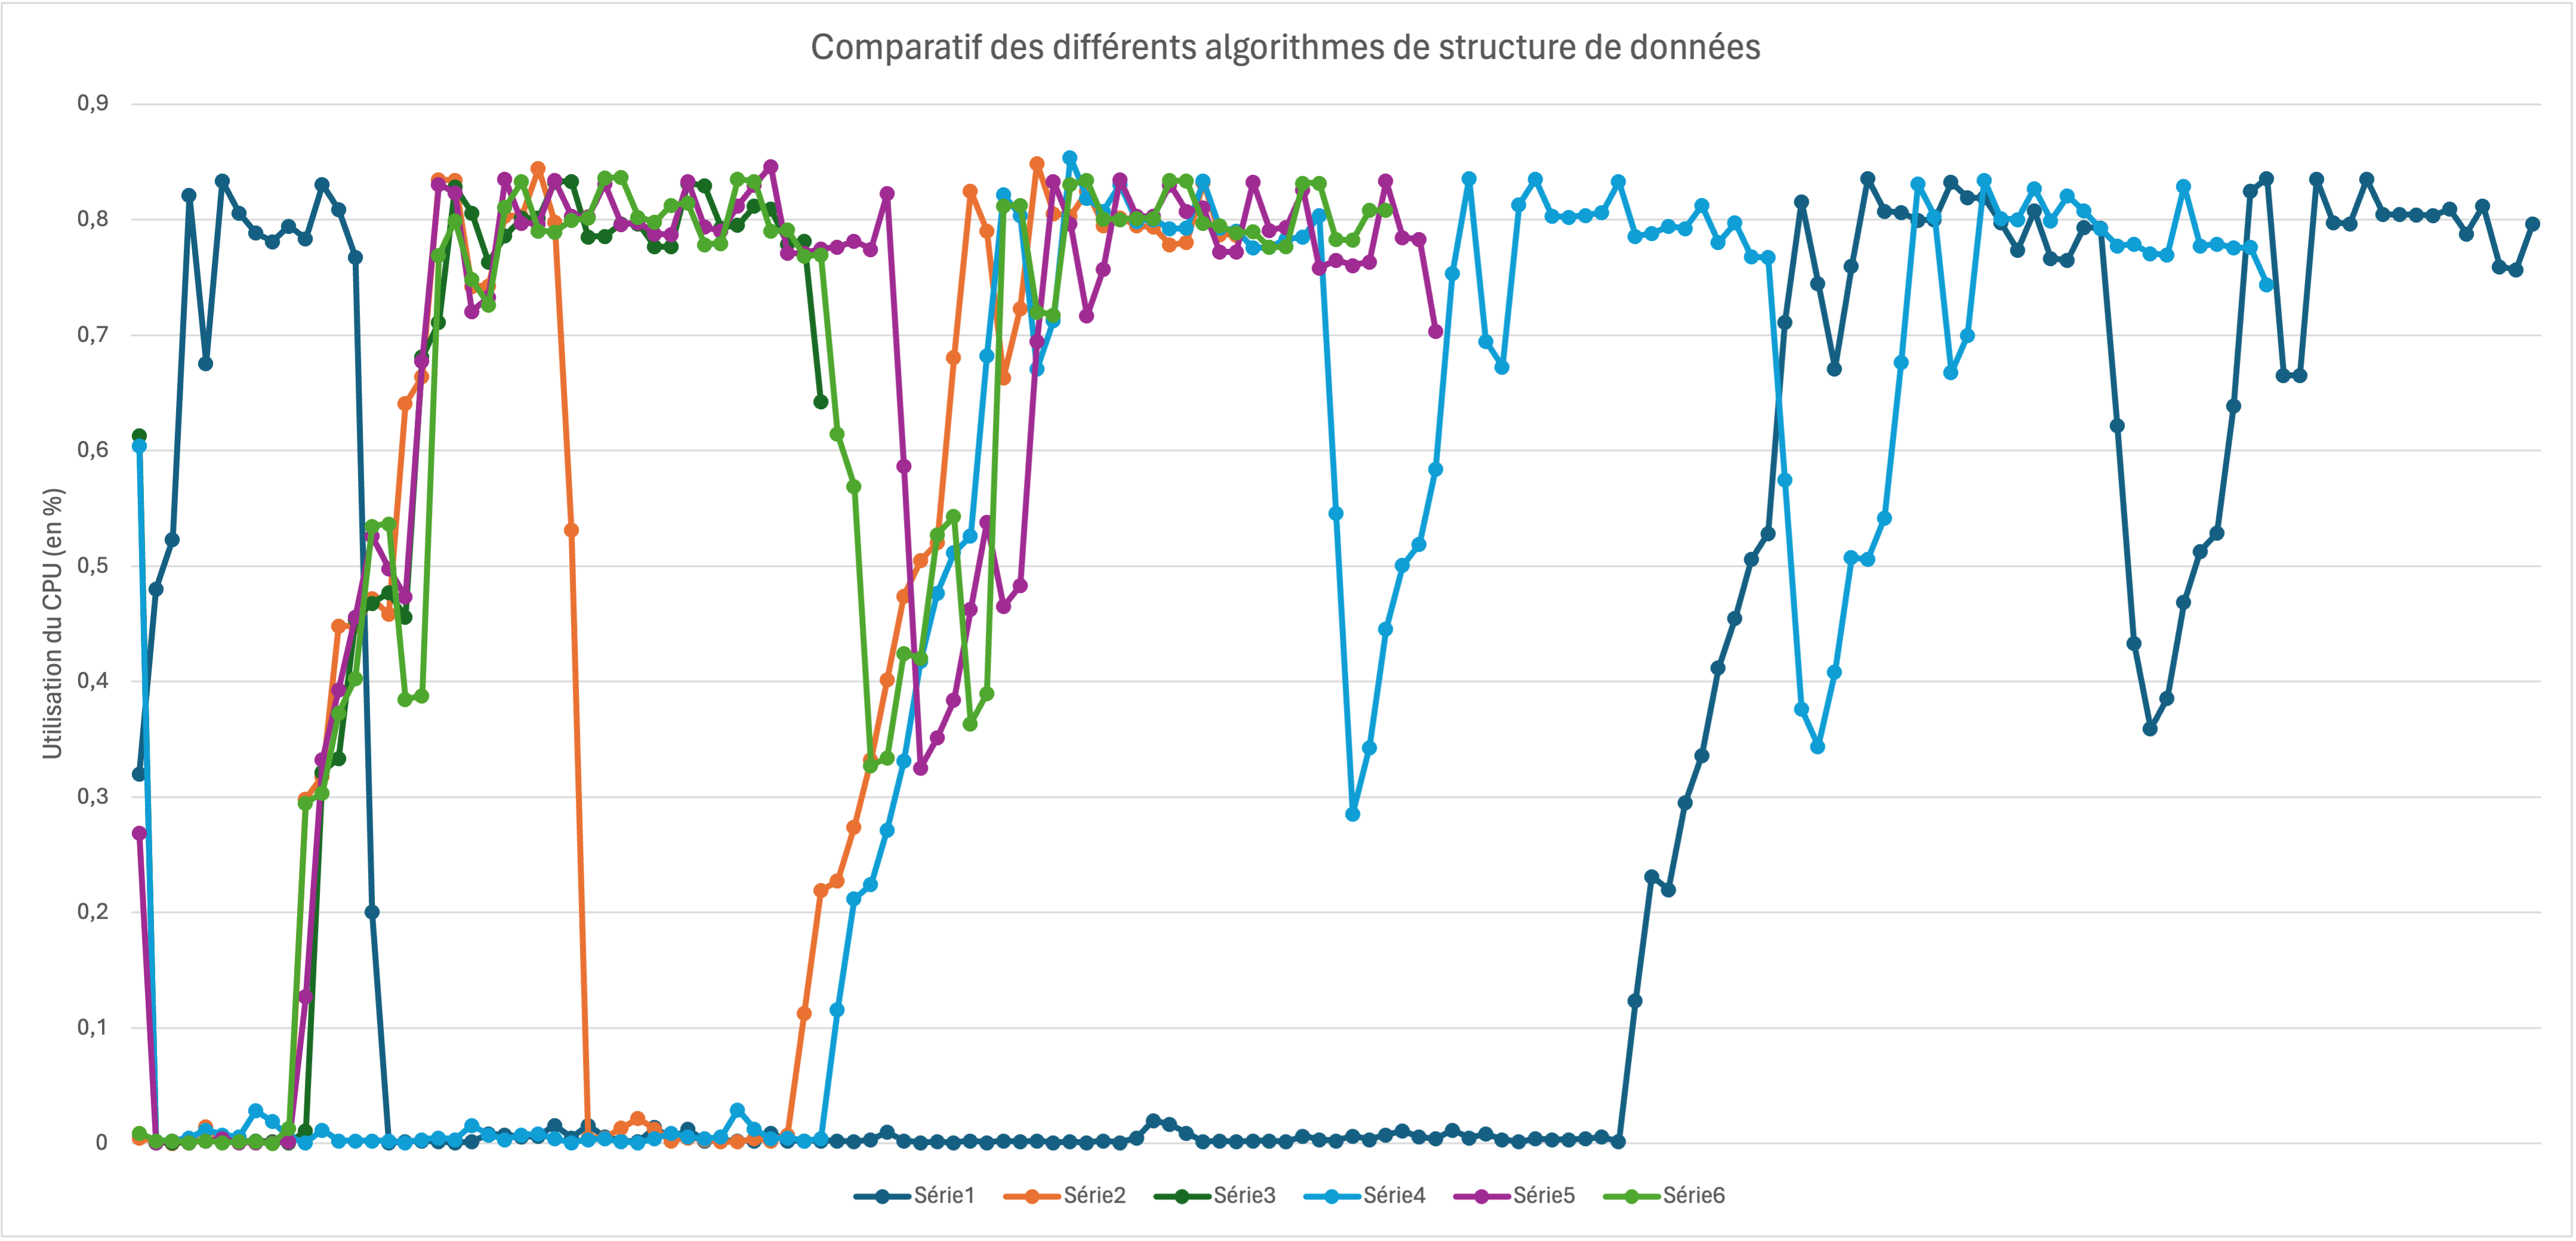
\includegraphics[width=1\linewidth]{res/graph/Datastructure/cpuuse_datastruct.png}
    \caption{Utilisation du CPU par les 6 programme de structure de données}
    \label{fig:cpuuse_datastruct}
\end{figure}
\begin{figure}[H]
    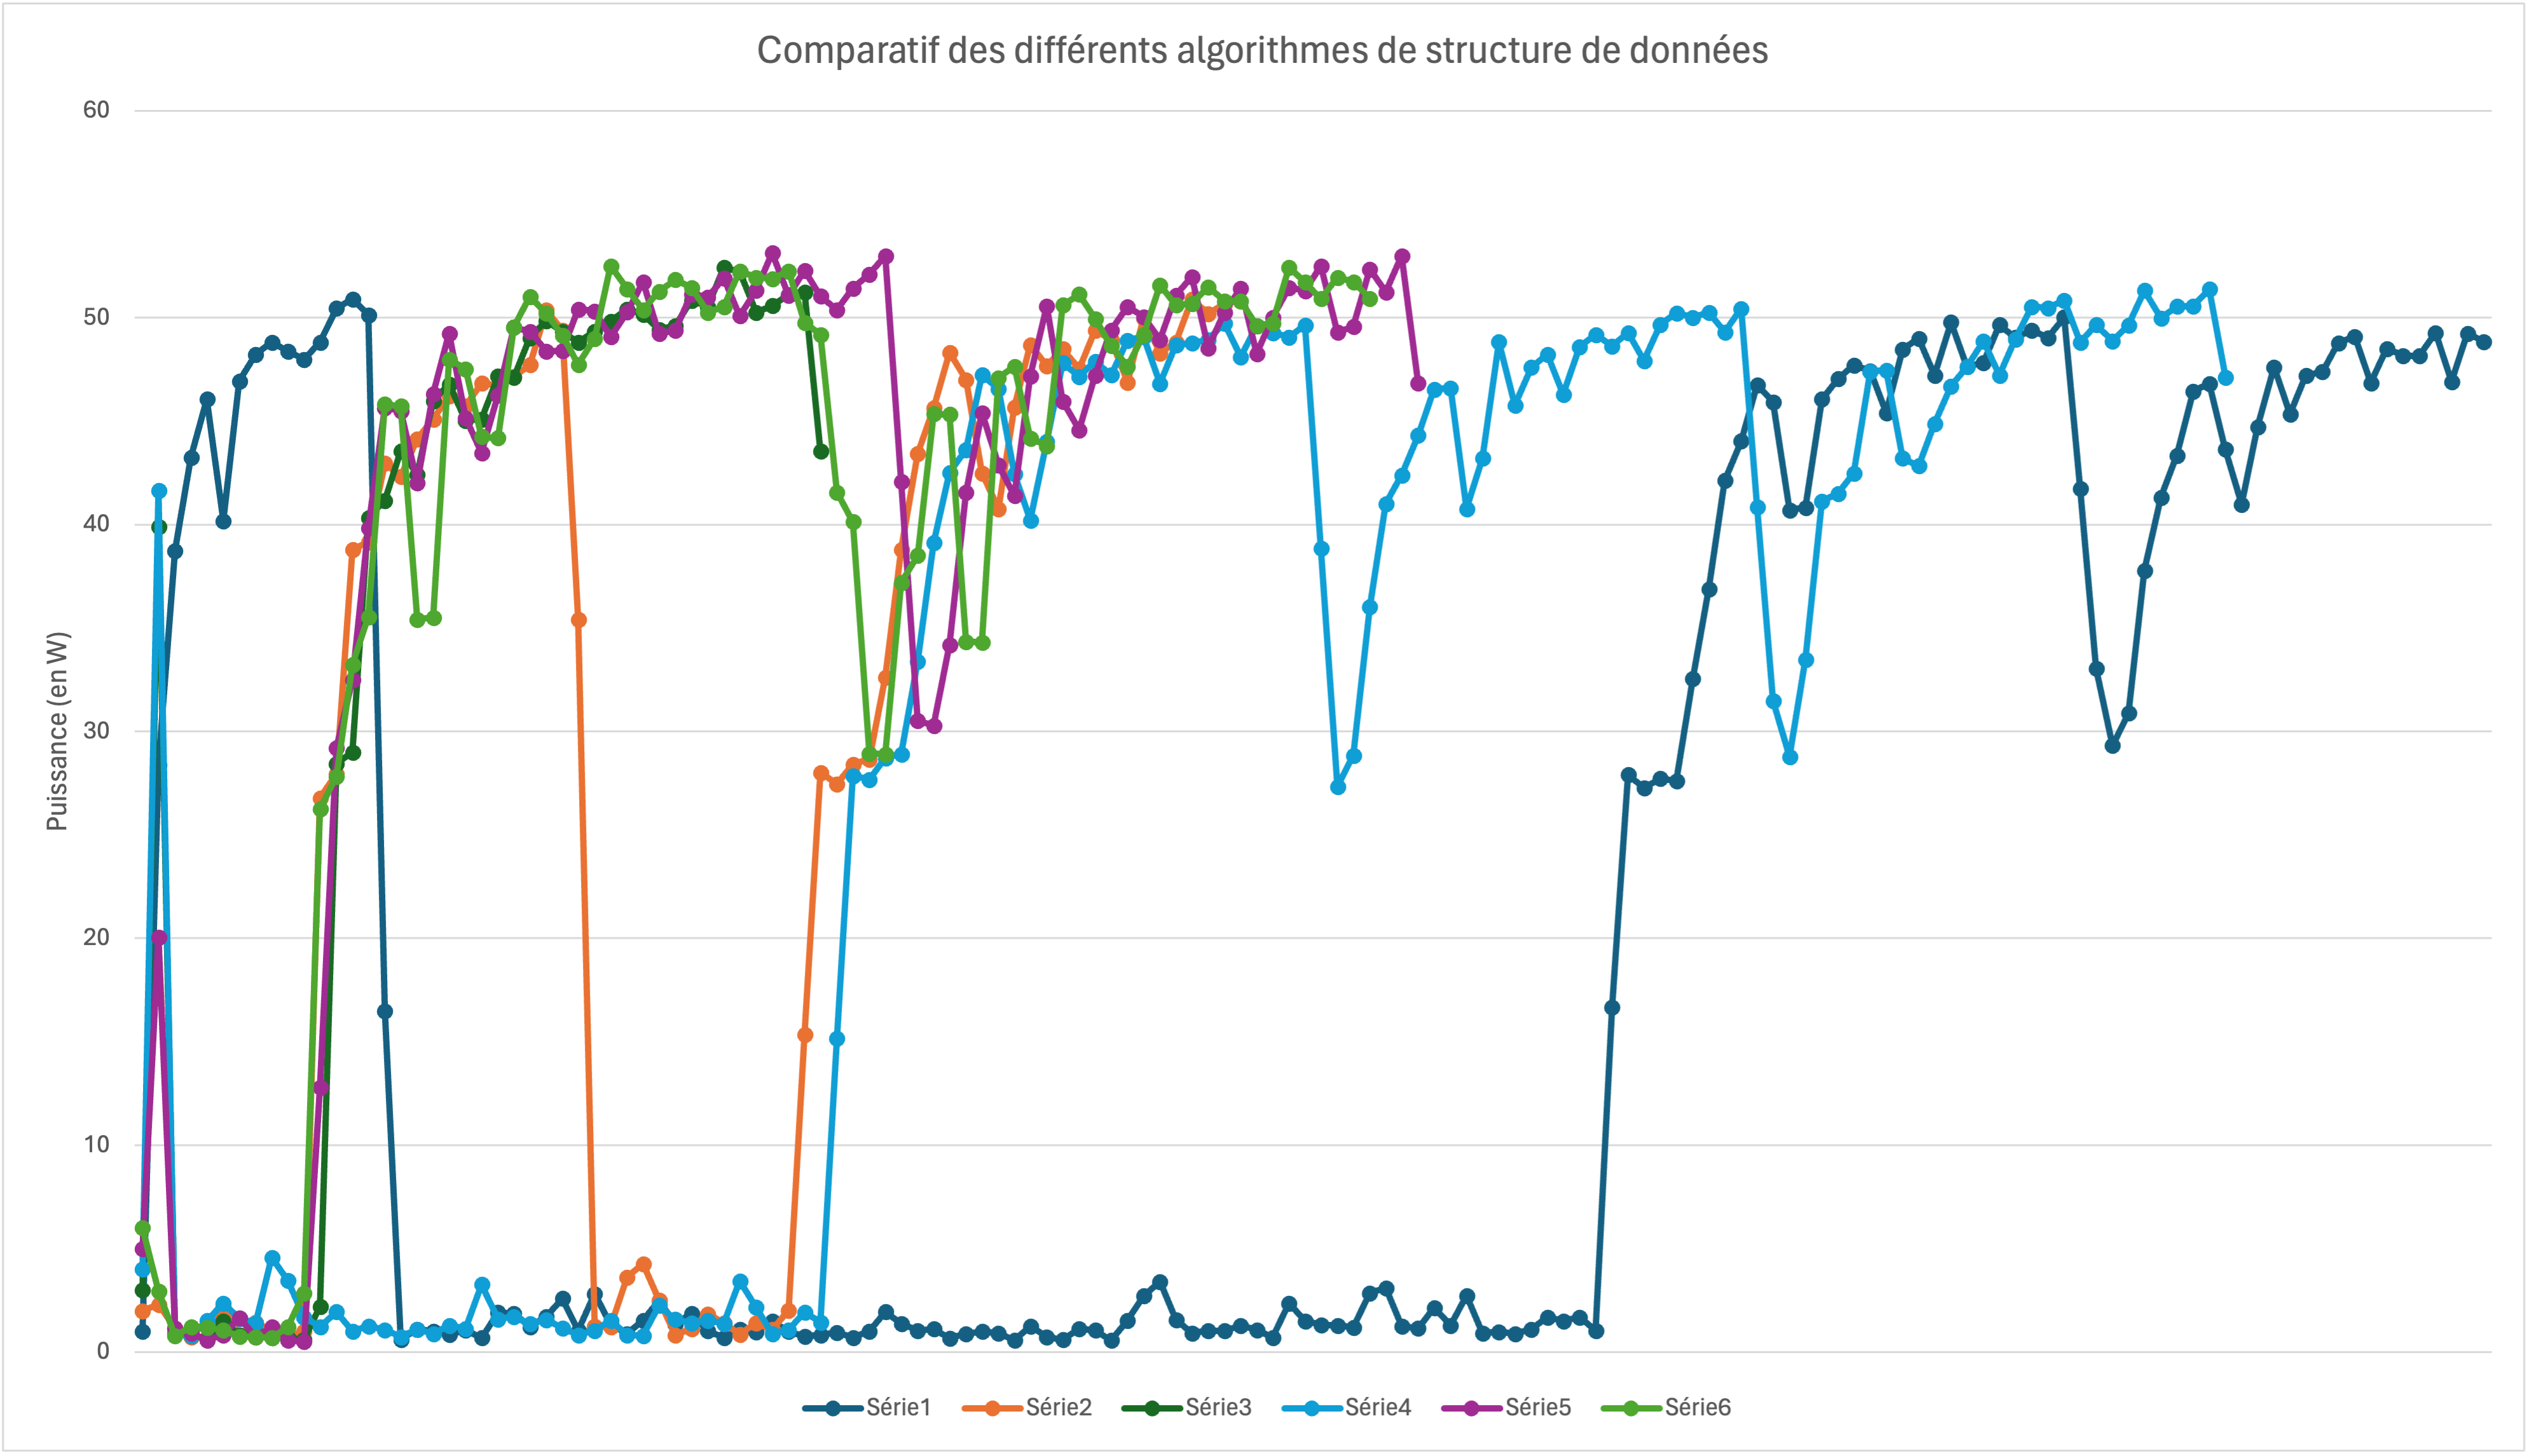
\includegraphics[width=1\linewidth]{res/graph/Datastructure/power_datastruct.png}
    \caption{Consommation totale de la puissance pour chaque programme de structure de données}
    \label{fig:power_datastruct}
\end{figure}

Comme nous pouvons le voir sur ces deux graphiques, la consommation et le pourcentage du CPU utilisé varie selon les programmes mais tend à suivre une certaine \textit{structure} pour les 6 programmes. Une montée haute, suivie d'une courte stabilisation avant de remonter vers la limite qui tourne à environ 50W ou 80\% de l'utilisation du CPU.
Cependant, la différence entre tous ces programmes et le moment ou se produit cette montée. Certains programmes auront cette montée beaucoup plus tard dans leur runtime, alors que d'autres ont ce pic très tôt. Il est cependant intéressant de noter que ces programmes \textit{rapide} ont tendance à finir leurs tâches plus tôt.
Malheureusement, pas contrainte de temps et personnels, nous n'aurons pas eu le temps de pousser cette étude statistique plus loin pour montrer quels programmes consomment le plus.

\subsection{Ray Casting en Java & C}
Pour cette deuxième expérience, nous avons expérimenter sur un même algorithme dans deux languages différents. (Nous n'auraons encore une fois pas eu le temps d'expérimenter avec d'autres languages comme initialement prévue.)
L'algorithme de Ray Casting est :
\begin{quote}
    Given a point and a polygon, check if the point is inside or outside the polygon using the ray-casting algorithm.
\end{quote}\cite{wiki:xxx}

\subsubsection{Version Java}
Voici les résultats pour la version Java :
\begin{figure}[H]
    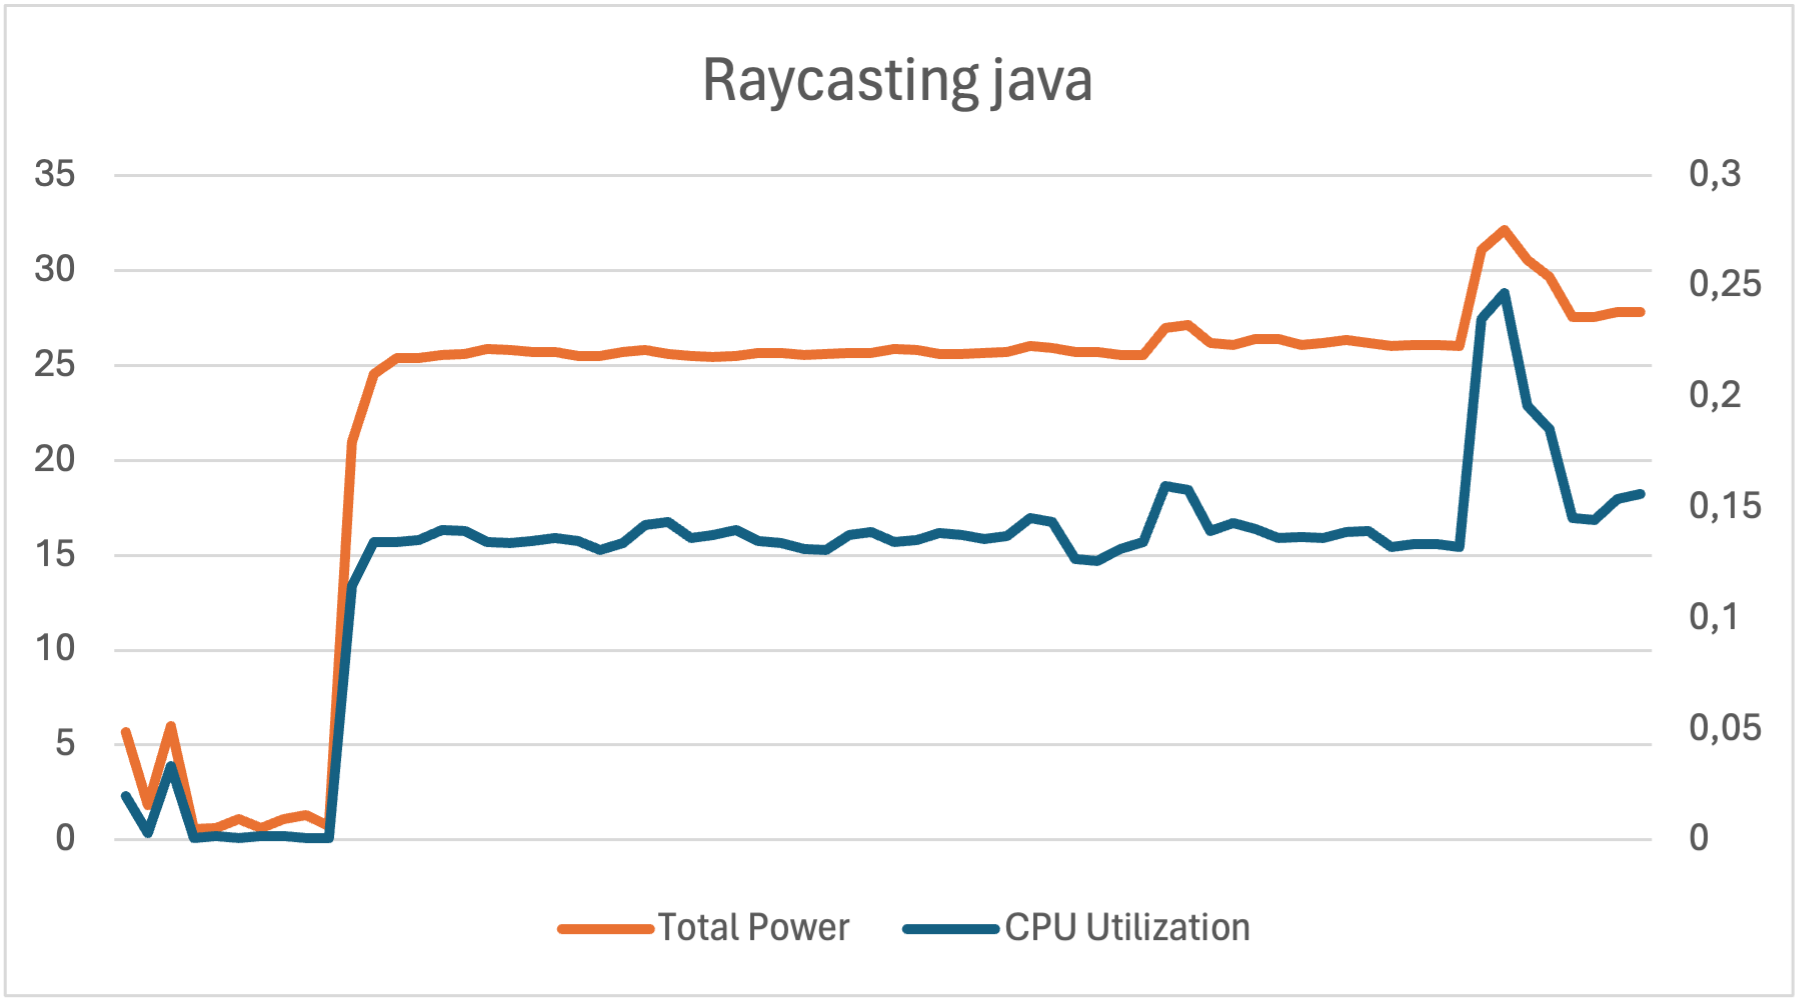
\includegraphics[width=1\linewidth]{res/graph/Raycasting/raycasting java.png}
    \caption{Performance de l'algorithme de Ray Casting en Java}
    \label{fig:java_raycasting}
\end{figure}

Un peu comme nos tests sur les programmes de structure de données, nous pouvon retrouver cette forme des courbes avec le premier pic, une stabilisation, un deuxième pic avant d'atteindre les limites où les courbes oscillent. 
Et nous avons une nouvelle fois une cohérence entre l'utilisation du CPU et la puissance consommée.

\subsubsection{Version C}
Voici les résultats pour la version C :
\begin{figure}[H]
    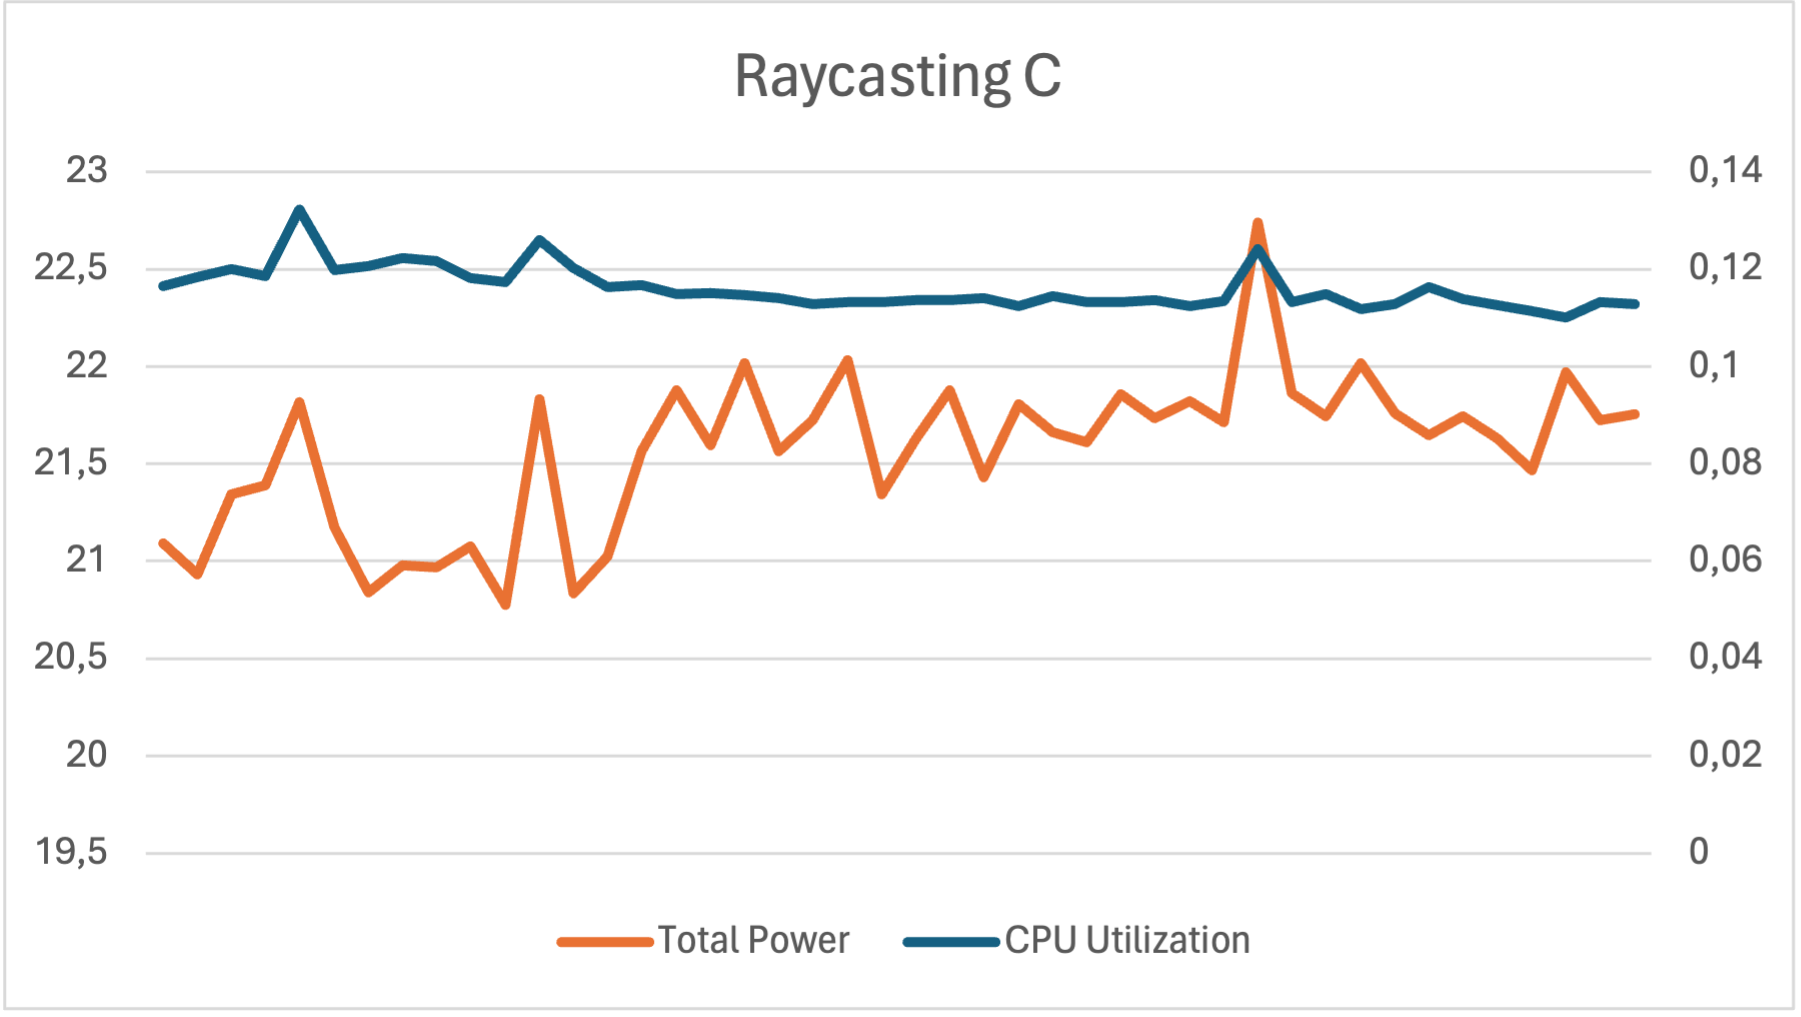
\includegraphics[width=1\linewidth]{res/graph/Raycasting/raycasting c.png}
    \caption{Performance de l'algorithme de Ray Casting en C}
    \label{fig:c_raycasting}
\end{figure}

Ici nous avons une bien grande différence avec le reste de nos résultats. La consommation et le pourcentage du CPU utilisé sont beaucoup plus constant à travers l'entiéreté de la vie du programme. Surtout au niveau du pourcentage d'utilisation du CPU.

Voici un graphique combinant les deux résultats :
\begin{figure}[H]
    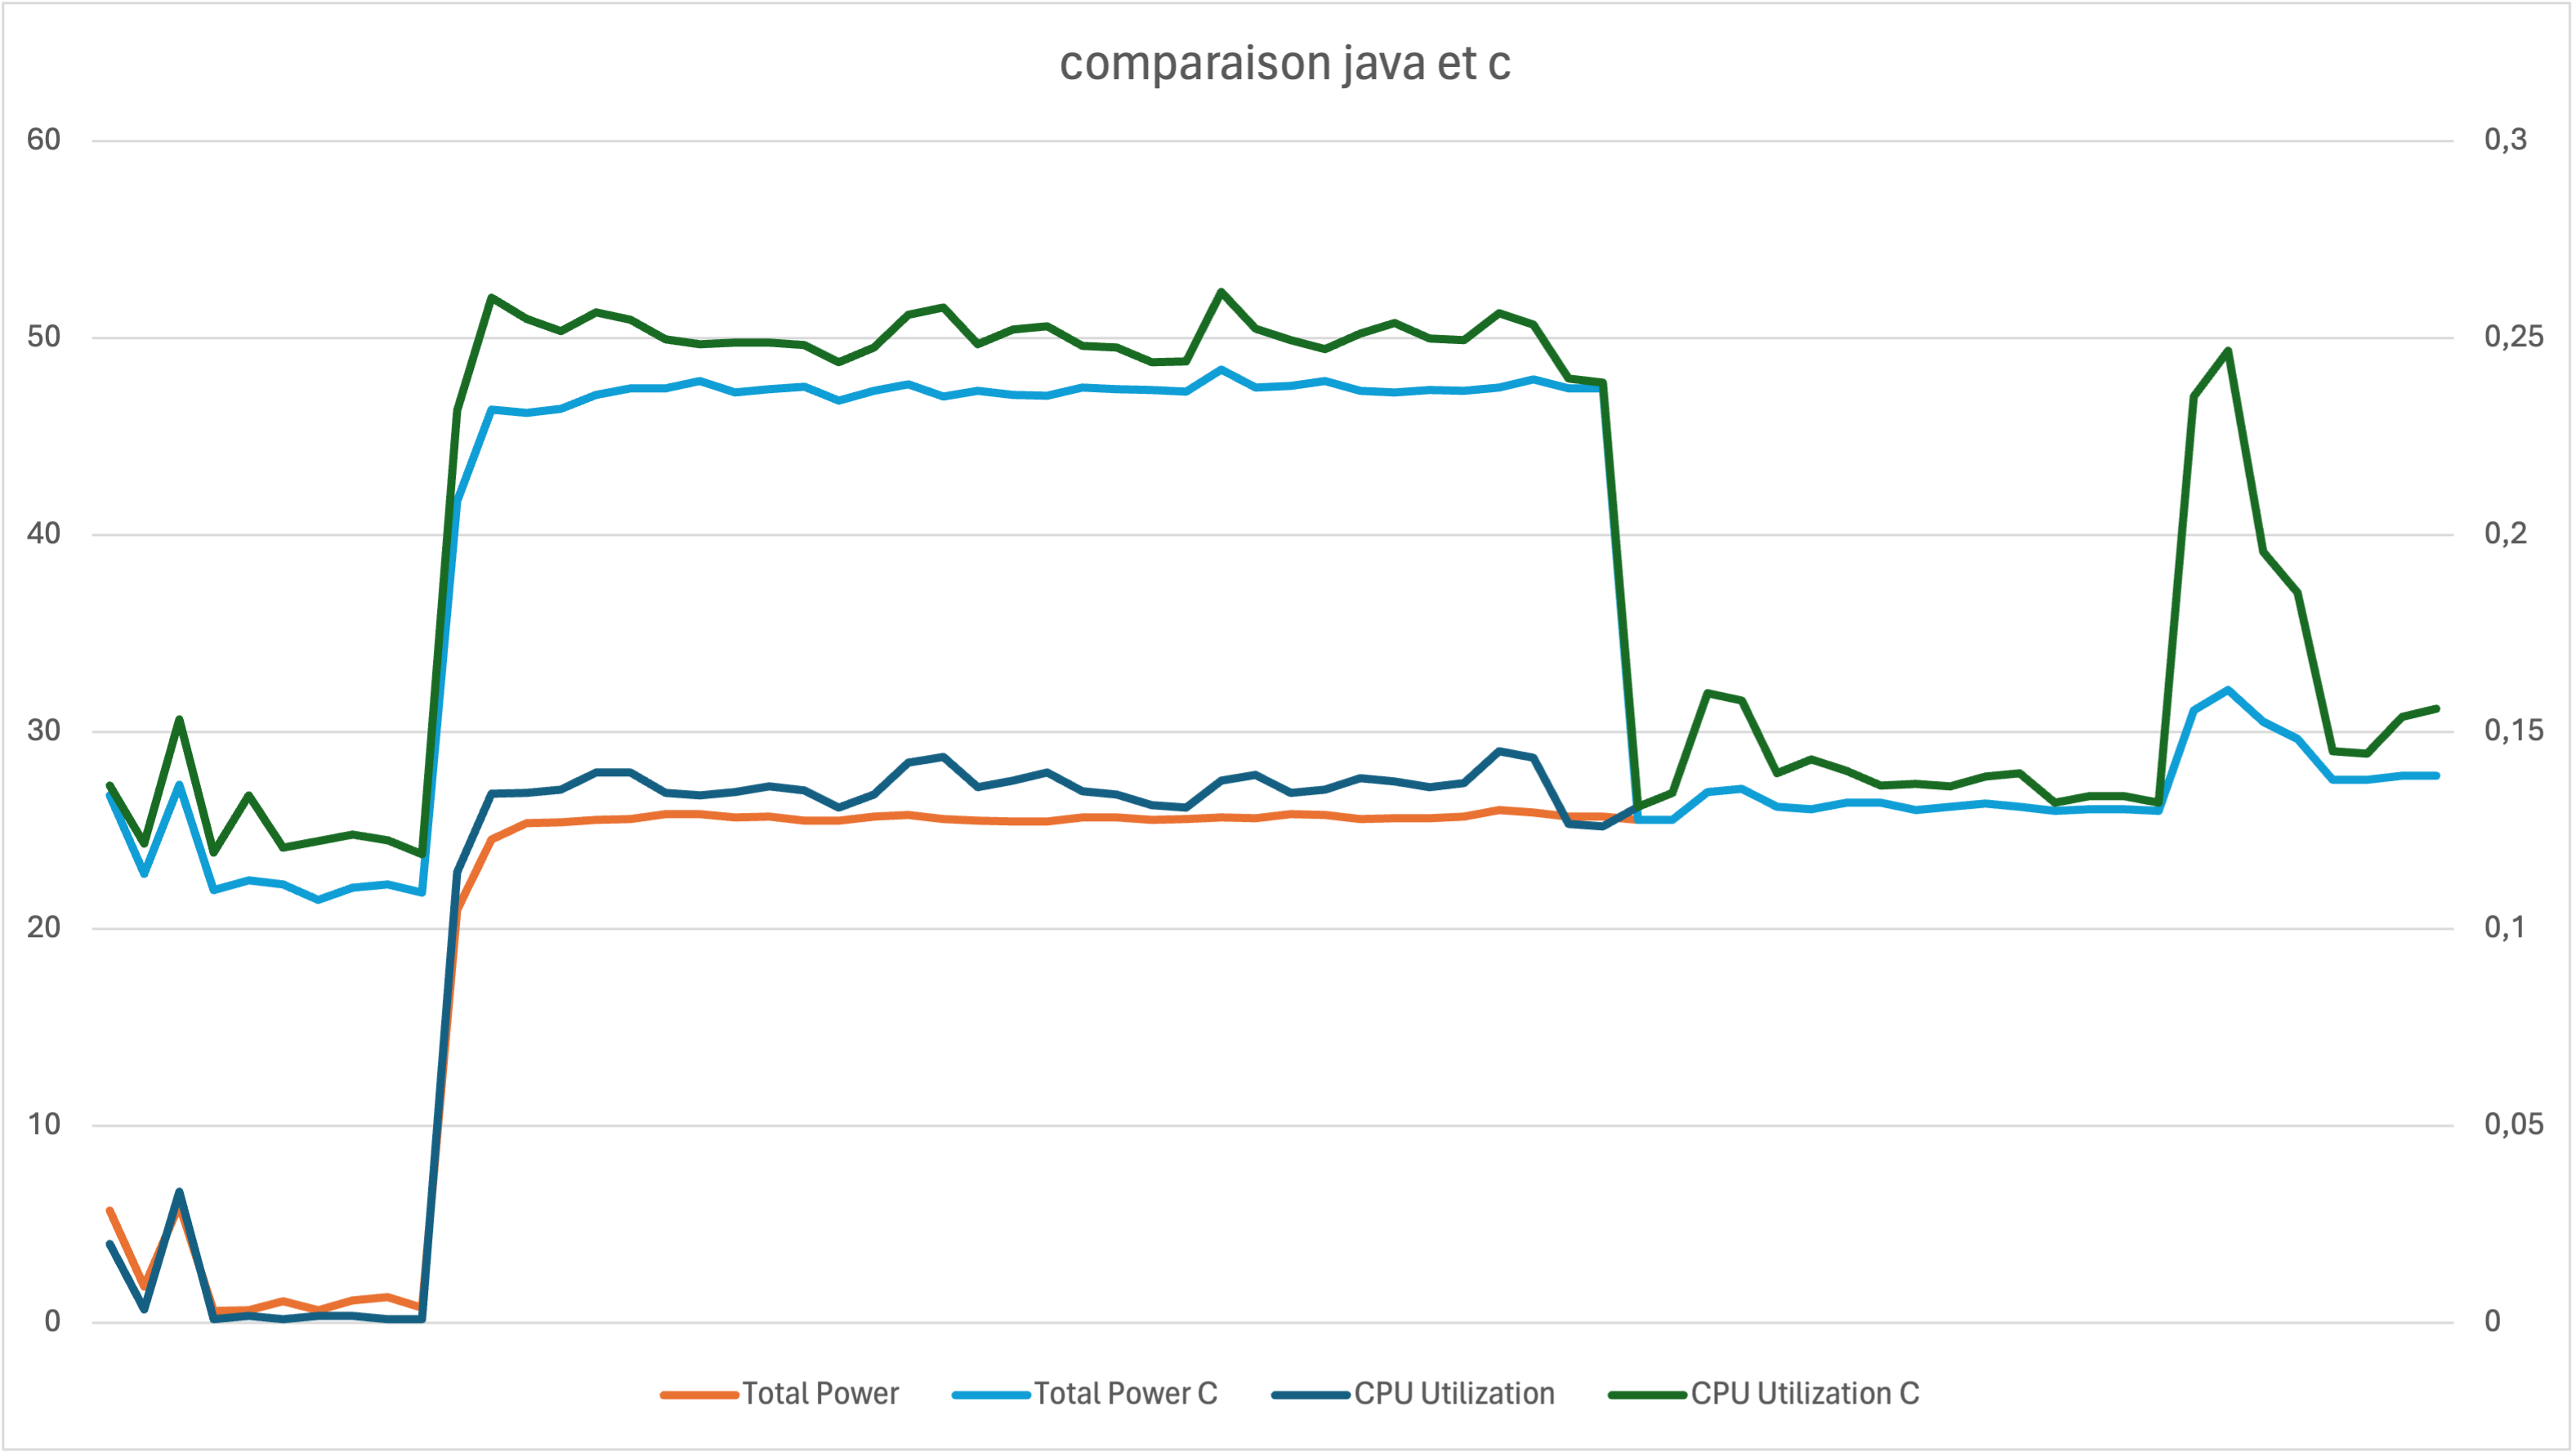
\includegraphics[width=1\linewidth]{res/graph/Raycasting/raycasting_combined.png}
    \caption{Graphique des résultats combiné}
    \label{fig:raycasting_combined}
\end{figure}

Nous pouvons voir ici que dès le départ, la version en C consomme beaucoup plus de puissance et d'utilisation du CPU comparé au programme en Java.

\chapter{\centering Conclusion}
Nous avons donc une nette différence notable entre la version Java et C du programme de Ray Casting. Pour ce genre d'algorithme, l'utilisation de Java est préférable car le language est mieux équipé pour s'attaquer à ce genre de problématique.
Cependant, il reste important de se souvenir que dans certains cas, le language C pourrait être préférable à C. Et nous ne prenons en compte ici que deux languages différents mais qui reste assez lié entre eux.

\bibliographystyle{plain}
\bibliography{ref}
\printglossary




\end{document}